\documentclass{article}
\usepackage{tikz, comment}
\usepackage{pifont}
\usepackage{fontspec}
\usetikzlibrary{arrows, decorations.markings, decorations.pathreplacing}
\begin{comment}
:Title: Not defined yet
:Tags: area using polar coordinates, polar integral formula ;polar form of a complex number;sohcahtoa;cosine, cos ;arc of a circle
:Prob: 0.4373;0.3842;0.3712;0.3507;0.3315
:Slug: No name yet

Description Here.........
\end{comment}
\begin{document}\centering

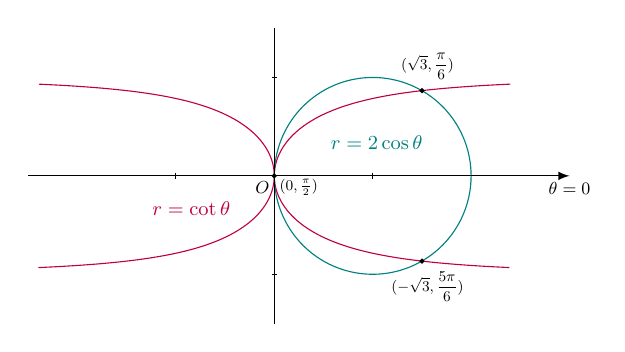
\begin{tikzpicture}[>=latex,xscale=.5*2.5, yscale=.5*2.5][font=\sf\small]

%\draw[xstep=1cm,ystep=1cm,color=gray!80] (0, -1) grid (8, 8);

\draw[purple, samples=100, smooth, domain=pi/2-1.2:pi/2+1.2, variable=\t]
plot ({cos(\t r)/sin(\t r)*cos(\t r)}, {cos(\t r)/sin(\t r)*sin(\t r)});

\draw[purple, samples=100, smooth, domain=3*pi/2-1.2:3*pi/2+1.2, variable=\t]
plot ({cos(\t r)/sin(\t r)*cos(\t r)}, {cos(\t r)/sin(\t r)*sin(\t r)});

\draw[teal, samples=100, smooth, domain=0:2*pi, variable=\t]
plot ({(2*cos(\t r))*cos(\t r)}, {(2*cos(\t r))*sin(\t r)});

\node[purple, xshift=-30, yshift=-12, scale=0.8] at (0,0) {$r=\cot\theta$};
\node[teal, xshift=37, yshift=12, scale=0.8] at (0,0) {$r=2\cos\theta$};

\draw[fill, xscale=1/2.5, yscale=1/2.5] ({0*2.5}, {0*2.5}) circle(0.05)node[right, xshift=0, yshift=-4, scale=0.6]{$(0, \frac{\pi}{2})$};

\draw[fill, xscale=1/2.5, yscale=1/2.5] ({(2*cos((pi/6) r))*cos((pi/6) r)*2.5}, {(2*cos((pi/6) r))*sin((pi/6) r)*2.5}) circle(0.05)node[above, xshift= 2, yshift= 2, scale=0.6]{$\displaystyle (\sqrt 3, \frac{\pi}{6})$};

\draw[fill, xscale=1/2.5, yscale=1/2.5] ({(2*cos((5*pi/6) r))*cos((5*pi/6) r)*2.5}, {(2*cos((5*pi/6) r))*sin((5*pi/6) r)*2.5}) circle(0.05)node[below, xshift= 2, yshift= -2, scale=0.6]{$\displaystyle (-\sqrt 3, \frac{5\pi}{6})$};

\foreach \x in {-1,1}
\draw (\x,2pt/2.5) -- (\x,-2pt/2.5)
node[anchor=north] {}%{\tiny$\x$}
;
\foreach \x in {}
\draw (\x,2pt/1.25) -- (\x,-2pt/1.25)
node[anchor=south] {\tiny$\x$}
;
\foreach \y in {-1,1}
\draw (-2pt/2.5,\y) -- (2pt/2.5,\y)
node[anchor=east] {}%{\tiny $\y$}
;

\draw[->] (-2.5, 0) -- (3, 0)node[below, scale=0.7] {$\theta=0$};
\draw[] (0, -1.5) -- (0, 1.5);

\node[scale=0.7] at (-0.3/2.5, -0.3/2.5) {$O$};

\end{tikzpicture}
\end{document}